\def\codent{\hskip 1.0em} % <- 'tab' for indentation.
\def\:{\mathrel{:\mathord=}}

\section{Relevance of Quintic Splines}

Many domains of science rely on smooth approximations to real-valued
functions over a closed interval. Piecewise polynomial functions
(splines) provide the smooth approximations for animation in graphics
\cite{herman2006techniques,quint2003scalable}, aesthetic structural support in
architecture \cite{brennan2020measure}, efficient aerodynamic surfaces in
automotive and aerospace engineering \cite{brennan2020measure}, prolonged
effective operation of electric motors \cite{berglund2009planning}, and
accurate nonparametric approximations in statistics \cite{knott2000interpolating}.
While polynomial interpolants and regressors apply broadly,
splines are often a good choice because they can approximate globally
complex functions while minimizing the local complexity of an
approximation.

It is often the case that the true underlying function or phenomenon
being modeled has known properties like convexity, positivity, various
levels of continuity, or monotonicity. Given a reasonable amount of
data, it quickly becomes difficult to achieve desirable properties in
a single polynomial function. In general, the maintenance of function
properties through interpolation/regression is referred to as
{\it shape preserving} \cite{fritsch1980monotone,gregory1985shape}.
The specific properties the present algorithm will preserve in
approximations are monotonicity and $C^2$ continuity. In addition to
previously mentioned applications, these properties are crucially
important in statistics to the approximation of a cumulative
distribution function and subsequently the effective generation of
random numbers from a specified distribution
\cite{ramsay1988monotone}.  A spline function with these properties
could approximate a cumulative distribution function to a high level
of accuracy with relatively few intervals. A twice continuously
differentiable approximation to a cumulative distribution function
(CDF) would produce a corresponding probability density function (PDF)
that is continuously differentiable, which is desirable.

The currently available software for monotone piecewise polynomial
interpolation includes quadratic \cite{he1998monotone},
cubic \cite{fritsch1980monotone}, and (with limited application) quartic
\cite{wang2004rational,abd2011improved,yao2018unconditionally} cases. In
addition, a statistical method for bootstrapping the construction of
an arbitrarily smooth monotone fit exists \cite{leitenstorfer2007generalized},
but the method does not take advantage of known analytic
properties of quintic polynomials. The code by Fritsch \cite{fritsch1982piecewise} for
$C^1$ cubic spline interpolation is the predominantly utilized code
for constructing monotone interpolants at present. Theory has been
provided for the quintic case \cite{ulrich1994positivity,hess1994positive}
and that theory was recently utilized in a proposed
algorithm \cite{lux2020algorithm} for monotone quintic spline construction, however
no published mathematical software exists.

The importance of piecewise quintic interpolation over lower order
approximations can be simply observed. In general, the order of a
polynomial determines the number of function (and derivative) values
it can interpolate, which in turn determines the growth rate of error
away from interpolated values. $C^2$ quintic (order six) splines
match the function value and two given derivatives at each breakpoint.
This work provides a Fortran 2003 subroutine {\tt MQSI} based on the
necessary and sufficient conditions in Ulrich and Watson \cite{ulrich1994positivity} for the
construction of monotone quintic spline interpolants of monotone data.
Precisely, the problem is, given a strictly increasing sequence $X_1<X_2<
\cdots <X_n$ of breakpoints with corresponding monotone increasing
function values $Y_1\le Y_2\le \cdots \le Y_n$, find a $C^2$ monotone
increasing quintic spline $Q(x)$ with the same breakpoints satisfying
$Q(X_i)=Y_i$ for $1\le i\le n$. ({\tt MQSI} actually does something slightly
more general, producing $Q(x)$ that is monotone increasing (decreasing)
wherever the data is monotone increasing (decreasing).)

The remainder of this chapter is structured as follows: Section 2 provides
the algorithms for constructing a $C^2$ monotone quintic spline interpolant
to monotone data, Section 3 outlines the method of spline representation
($B$-spline basis) and evaluation, Section 4 analyzes the complexity and
sensitivity of the algorithms in {\tt MQSI}, and Section 5 presents an
empirical performance study and some graphs of constructed interpolants.

\section{Monotone Quintic Interpolation}

In order to construct a monotone quintic interpolating spline, two
primary problems must be solved. First, reasonable derivative values
at data points need to be estimated. Second, the estimated derivative
values need to be modified to enforce monotonicity on all polynomial
pieces.

Fritsch and Carlson \cite{fritsch1980monotone} originally proposed the use of central differences
to estimate derivatives, however this often leads to extra and unnecessary
{\it wiggles} in the spline when used to approximate second derivatives.
In an attempt to capture the local shape of the data, this package uses a
facet model from image processing \cite{haralick1981facet} to estimate
first and second derivatives at breakpoints. Rather than picking a local
linear or quadratic fit with minimal residual, this work uses a quadratic
facet model that selects the local quadratic interpolant with minimum
magnitude curvature.

\begin{plain}
\parskip=0pt
%% ===================================================================
%%                   Algorithm 1: QUADRATIC_FACET
\vskip 5mm
{\parindent 0mm
{\bf Algorithm 1:} {
\tt QUADRATIC\_FACET}$\bigl(X(1{:}n)$, $Y(1{:}n)$, $i \bigr)$

where $X_j$, $Y_j$ $\in \mathbb{R}$ for $j = 1$, $\ldots$, $n$, $1 \le i
\le n$, and $n \ge 3$. Returns the slope and curvature at $X_i$ of the
local quadratic interpolant with minimum magnitude curvature.

}
{\parindent=3mm
%% -------------------------------------------------------------------
\item{} {\tt if} $\bigl((i\ne1\wedge Y_i \approx Y_{i-1})$ {\tt or}
$(i\ne n\wedge Y_i \approx Y_{i+1})\bigr)$ {\tt then return $(0,0)$}

\item{} {\tt else if} $i=1$ {\tt then}
\itemitem{} $f_1\:\hbox{interpolant to }(X_1,Y_1)$,
  $(X_2,Y_2)$, and $(X_3,Y_3)$.
\itemitem{} {\tt if} $\bigl(Df_1(X_1)(Y_2-Y_1)<0\bigr)$ {\tt then return}
  $\bigl(0,0\bigr)$
\itemitem{} {\tt else return} $\bigl(Df_1(X_1),D^2f_1\bigr)$
\itemitem{} {\tt endif}

\item{} {\tt else if} $i=n$ {\tt then}
\itemitem{} $f_1\:\hbox{interpolant to }(X_{n-2},Y_{n-2})$,
  $(X_{n-1},Y_{n-1})$, and $(X_n,Y_n)$.
\itemitem{} {\tt if} $\bigl(Df_1(X_n)(Y_n-Y_{n-1})<0\bigr)$ {\tt then return}
  $\bigl(0,0\bigr)$
\itemitem{} {\tt else return} $\bigl(Df_1(X_n),D^2f_1\bigr)$
\itemitem{} {\tt endif}

\item{} {\tt else if} $\bigl(1<i<n\wedge (Y_{i+1} - Y_i)(Y_i - Y_{i-1}) < 0
\bigr)$ {\tt then}
\itemitem{} The point $(X_i$, $Y_i)$ is an extreme point. The
quadratic with minimum magnitude
curvature that has slope zero at $X_i$ will be the facet chosen.
\itemitem{} $f_1\:\hbox{interpolant to }(X_{i-1},Y_{i-1})$, $(X_i,Y_i)$,
  and $Df_1(X_i) = 0$.
\itemitem{} $f_2\:\hbox{interpolant to }(X_i,Y_i)$, $(X_{i+1},Y_{i+1})$,
  and $Df_2(X_i) = 0$.
\itemitem{} {\tt if} $\bigl(|D^2f_1| \leq |D^2f_2|\bigr)$ {\tt then
  return} $\bigl(0$, $D^2f_1\bigr)$
\itemitem{} {\tt else return} $\bigl(0$, $D^2f_2\bigr)$
\itemitem{} {\tt endif}

\item{} {\tt else}
\itemitem{} {The point $(X_i$, $Y_i)$ is in a monotone segment of
data. In the following, it is possible that $f_1$ or $f_3$ do
not exist because $i \in \{2, n-1\}$. In those cases, the minimum
magnitude curvature among existing quadratics is chosen.}
\itemitem{} $f_1\:\hbox{interpolant to }(X_{i-2},Y_{i-2})$,
  $(X_{i-1},Y_{i-1})$, and $(X_i,Y_i)$.
\itemitem{} $f_2\:\hbox{interpolant to }(X_{i-1},Y_{i-1})$,
  $(X_i,Y_i)$, and $(X_{i+1},Y_{i+1})$.
\itemitem{} $f_3\:\hbox{interpolant to }(X_i,Y_i)$,
  $(X_{i+1},Y_{i+1})$, and $(X_{i+2},Y_{i+2})$.

\itemitem{} {\tt if} $\bigl(Df_1(X_i)(Y_i-Y_{i-1}) \ge 0 \wedge
  |D^2f_1| = \min\bigl\{ |D^2f_1|,
  |D^2f_2|, |D^2f_3|\bigr\} \bigr)$ {\tt then}
\itemitem{} \codent {\tt return} $\bigl(Df_1(X_i),D^2f_1\bigr)$

\itemitem{} {\tt else if} $\bigl(Df_2(X_i)(Y_i-Y_{i-1}) \ge 0 \wedge
  |D^2f_2| = \min\bigl\{ |D^2f_1|,
  |D^2f_2|, |D^2f_3|\bigr\} \bigr)$ {\tt then}
\itemitem{} \codent {\tt return} $\bigl(Df_2(X_i),D^2f_2\bigr)$

\itemitem{} {\tt else if} $\bigl(Df_3(X_i)(Y_{i+1}-Y_i) \ge 0\bigr)$ {\tt then}
\itemitem{} \codent {\tt return} $\bigl(Df_3(X_i),D^2f_3\bigr)$
\itemitem{} {\tt else return} $(0, 0)$
\itemitem{} {\tt endif}
\item{} {\tt endif}
}
\vskip 5mm
%% ----------------------------------------------------------------------
\end{plain}

The estimated derivative values by the quadratic facet model are not
guaranteed to produce monotone quintic polynomial segments. Ulrich and
Watson \cite{ulrich1994positivity} established tight constraints on the monotonicity of a
quintic polynomial piece, while deferring to He{\ss} and Schmidt
\cite{hess1994positive} for a relevant simplified case. The following algorithm
implements a sharp check for monotonicity by considering the
nondecreasing case. The nonincreasing case is handled similarly.

\begin{plain}
\parskip=0pt
%% ===================================================================
%%                    Algorithm 2: IS_MONOTONE
\vskip 5mm
{\parindent 0mm
{\bf Algorithm 2:}

{\tt IS\_MONOTONE}$\bigl(x_0$, $x_1$, $f(x_0)$, $Df(x_0)$,
$D^2f(x_0)$, $f(x_1)$, $Df(x_1)$, $D^2f(x_1) \bigr)$

where $x_0$, $x_1 \in {\mathbb R}$, $x_0 < x_1$, and $f$ is an order six
polynomial defined by $f(x_0)$, $Df(x_0)$, $D^2f(x_0)$, $f(x_1)$,
$Df(x_1)$, $D^2f(x_1)$. Returns {\tt TRUE} if $f$ is monotone
increasing on $[x_0,x_1]$.

}
{\parindent=6mm
%% -------------------------------------------------------------------
\item{1.} {\tt if} $\bigl(f(x_0) \approx f(x_1)\bigr)$ {\tt then}
\item{2.} \codent {\tt return} $\bigl( 0 = Df(x_0) = Df(x_1)
  = D^2f(x_0) = D^2f(x_1) \bigr)$
\item{3.} {\tt endif}
\item{4.} {\tt if} $\bigl(Df(x_0) < 0$ {\tt or} $Df(x_1) < 0\bigr)$ {\tt
  then return FALSE endif}
\item{5.} $w \: x_1 - x_0$
\item{6.} $z \: f(x_1) - f(x_0)$

\item{} {The necessity of Steps 1--4 follows directly from the
  fact that $f$ is $C^2$. The following Steps 7--13 coincide with a
  simplified condition for quintic monotonicity that reduces to one of
  cubic positivity studied by Schmidt and He{\ss} [1988]. Given
  $\alpha$, $\beta$, $\gamma$, and $\delta$ as defined by Schmidt and
  He{\ss}, monotonicity results when $\alpha \geq 0$, $\delta \geq 0$,
  $\beta \geq \alpha - 2 \sqrt{\alpha \delta}$, and $\gamma \geq
  \delta - 2 \sqrt{\alpha \delta}$.  Step 4 checked for $\delta < 0$,
  Step 8 checks $\alpha < 0$, Step 10 checks $\beta < \alpha - 2
  \sqrt{\alpha \delta}$, and Step 11 checks $\gamma < \delta - 2
  \sqrt{\alpha \delta}$. If none of the monotonicity conditions are
  violated, then the order six piece is monotone and Step 12
  concludes.}

\item{7.} {\tt if} $\bigl(Df(x_0) \approx 0$ {\tt or} $Df(x_1) \approx
0\bigr)$ {\tt then}
\item{8.} \codent {\tt if} $\bigl(D^2f(x_1)w > 4Df(x_1)$ {\tt then
return FALSE endif}
\item{9.} \codent $t \: 2 \sqrt{Df(x_0) (4Df(x_1) - D^2f(x_1) w) }$
\item{10.} \codent {\tt if} $\bigl(t + 3Df(x_0) + D^2f(x_0)w < 0 \bigr)$
  {\tt then return FALSE endif}
\item{11.} \codent {\tt if} $\bigl(60z - w\bigl(24Df(x_0) + 32Df(x_1) - 2t
  + w(3D^2f(x_0) - 5D^2f(x_1))\bigr) < 0\bigr)$
\item{}   \codent \codent {\tt then return FALSE endif}
\item{12.} \codent {\tt return TRUE}
\item{13.} {\tt endif}

\item{} {The following code considers the full quintic monotonicity
case studied by Ulrich and Watson \cite{ulrich1994positivity}. Given $\tau_1$, $\alpha$,
$\beta$, and $\gamma$ as defined by Ulrich and Watson, a quintic
piece is proven to be monotone if and only if
$\tau_1 > 0$, and $\alpha, \gamma > -(\beta+2)/2$ when $\beta \leq 6$,
and $\alpha, \gamma > -2 \sqrt{\beta-2}$ when $\beta > 6$.
Step 14 checks $\tau_1 \le 0$, Steps 19 and 20 determine monotonicity based
on $\alpha$, $\beta$, and $\gamma$.}

\item{14.} {\tt if} $\bigl( w\bigl(2\sqrt{Df(x_0)\,Df(x_1)} - 3(Df(x_0) +
  Df(x_1))\bigr) - 24z \leq 0 \bigr)$
\item{} \codent {\tt then return FALSE endif}
\item{15.} $t \: \bigl(Df(x_0)\, Df(x_1)\bigr)^{3/4}$
\item{16.} $\alpha \: (4 Df(x_1) - D^2f(x_1)w) \sqrt{Df(x_0)} / t$
\item{17.} $\gamma \: (4 Df(x_0) - D^2f(x_0)w) \sqrt{Df(x_1)} / t$
\item{18.} $\displaystyle \beta \: {60z/w + 3\bigl(w(D^2f(x_1) -
  D^2f(x_0)) - 8(Df(x_0) + Df(x_1))\bigr) \over 2 \sqrt{Df(x_0)\,Df(x_1)}}$
\item{19.} {\tt if} $(\beta \leq 6)$ {\tt then return}
$\bigl( \min\{\alpha,\gamma\} > - (\beta + 2) / 2 \bigr)$
\item{20.} {\tt else} {\tt return}
$\bigl( \min\{\alpha,\gamma\} > -2 \sqrt{\beta - 2}\,\bigr)$
\item{21.} {\tt endif}
}
\vskip 5mm
%% ----------------------------------------------------------------------
\end{plain}

It is shown by Ulrich and Watson \cite{ulrich1994positivity} that when $0 = DQ(X_i) =
DQ(X_{i+1}) = D^2Q(X_i) = D^2Q(X_{i+1})$, the quintic polynomial
over $[X_i$, $X_{i+1}]$ is guaranteed to be monotone. Using this fact, the
following algorithm shrinks (in magnitude) initial derivative estimates
until a monotone spline is achieved and outlines the core routine in the
accompanying package.

\begin{plain}
\parskip=0pt
%% ===================================================================
%%       Algorithm 3: MQSI - Monotone quintic spline interpolant
\vskip 3mm
{\parindent 0mm
{\bf Algorithm 3:} {\tt MQSI}$\bigl(X(1{:}n), Y(1{:}n) \bigr)$

where $(X_i,Y_i) \in \mathbb{R}\times\mathbb{R}$, $i = 1$, $\ldots$, $n$ are data
points. Returns monotone quintic spline interpolant $Q(x)$ such that
$Q(X_i) = Y_i$ and is monotone increasing (decreasing) on all
intervals that $Y_i$ is monotone increasing (decreasing).

}
{\parindent=6mm
\item{} Approximate first and second derivatives at $X_i$ with {\tt
  QUADRATIC\_FACET}.
\item{} {\tt for} $i\:1$ {\tt step} 1 {\tt until} $n$ {\tt do}
\item{} \codent $(u_i$, $v_i)\:$ {\tt QUADRATIC\_FACET}$(X$, $Y$, $i)$
\item{} {\tt enddo}
\item{} Identify and store all intervals where $Q$ is nonmonotone in a
queue $\cal Q$.
\item{} {\tt for} $i\:1$ {\tt step} 1 {\tt until} $n-1$ {\tt do}
\item{} \codent {\tt if not IS\_MONOTONE}$(X_i$, $X_{i+1}$, $Y_i$, $u_i$,
$v_i$, $Y_{i+1}$, $u_{i+1}$, $v_{i+1})$ {\tt then}
\item{} \codent\codent Add interval $\bigl(X_i$, $X_{i+1}\bigr)$ to
queue $\cal Q$.
\item{} \codent {\tt endif}
\item{} {\tt enddo}
\item{} {\tt do while} $\bigl($ queue $\cal Q$ of intervals is nonempty $\bigr)$
\itemitem{} Shrink (in magnitude) $DQ$ (in $u$) and $D^2Q$ (in $v$)
  that border intervals where $Q$ is nonmonotone.  
\itemitem{} Identify and store remaining intervals where $Q$ is
  nonmonotone in queue $\cal Q$.
\item{} {\tt enddo}
\item{} Construct and return a $B$-spline representation of $Q(x)$.
}
\vskip 3mm
%% ----------------------------------------------------------------------
\end{plain}

Since {\tt IS\_MONOTONE} can handle both nondecreasing and
nonincreasing simultaneously by taking into account the sign of $z$,
Algorithm 3 produces $Q(x)$ that is monotone increasing (decreasing)
over exactly the same intervals that the data $(X_i$, $Y_i)$ is
monotone increasing (decreasing).

Given the minimum magnitude curvature nature of the initial derivative
estimates, it is desirable to make the smallest necessary changes to
the initial interpolating spline $Q$ while enforcing monotonicity. In
practice a binary search for the boundary of monotonicity is used in
place of solely shrinking $DQ$ and $D^2Q$ at breakpoints adjoining
{\it active\/} intervals, or intervals over which $Q$ is nonmonotone at
least once during the search. The binary search considers a Boolean
function $B_i(s)$, for $0 \le s \le 1$, that is true if the order six
polynomial $Q(x)$ on $[X_i, X_{i+1}]$ matching derivatives
$Q(X_i)=Y_i$, $DQ(X_i)=s \,u_i$, $D^2Q(X_i)=s \,v_i$ at $X_i$, and derivatives
$Q(X_{i+1})=Y_{i+1}$, $DQ(X_{i+1})=s \,u_{i+1}$, $D^2Q(X_{i+1})=s \,v_{i+1}$
at $X_{i+1}$ is monotone, and false otherwise. As is outlined in Algorithm
3, the binary search is only applied at those breakpoints adjoining intervals
$[X_i, X_{i+1}]$ over which $Q$ is nonmonotone and hence $B_i(1)$ is false.
It is further assumed that there exists $0 \le s^* \le 1$ such that $B_i(s)$
is true for $0 \le s \le s^*$ and false for some $1 > s > s^*$. Since the
derivative conditions at interior breakpoints are shared by intervals left
 and right of the breakpoint, the binary search is performed at all
breakpoints simultaneously.  Specifically, the monotonicity of $Q$ is
checked on all active intervals in each step of the binary search to
determine the next derivative modification at each breakpoint. The goal
of this search is to converge on the boundary of the monotone region in
the $(\tau_1$, $\alpha$, $\beta$, $\gamma)$ space (described in Ulrich and
Watson \cite{ulrich1994positivity}) for all intervals. This multiple-interval binary search
allows the value zero to be obtained for all (first and second) derivative
values in a fixed number of computations, hence has no effect on
computational complexity order. This binary search algorithm is outlined
below.

\begin{plain}
\parskip=0pt
%% ===================================================================
%%              Algorithm 4: Global binary search
\vskip 5mm {\parindent 0mm {\bf Algorithm 4:} {\tt
    BINARY\_SEARCH}$\bigl(X(1{:}n), Y(1{:}n), u(1{:}n), v(1{:}n) \bigr)$

where $(X_i,Y_i) \in \mathbb{R}\times\mathbb{R}$, $i = 1$, $\ldots$, $n$ are
data points, and $Q(x)$ is a quintic spline interpolant such that
$Q(X_i) = Y_i$, $DQ(X_i) = u_i$, $D^2Q(X_i) = v_i$. Modifies
derivative values ($u$ and $v$) of $Q$ at data points to ensure
{\tt IS\_MONOTONE} is true for all intervals defined by adjacent data
points, given a desired precision $\mu \in {\mathbb R}$. proj$\bigl(w$,
int$(a,b)\bigr)$ denotes the projection of $w$ onto the closed
interval with endpoints $a$ and $b$.

}
{\parindent=6mm
\item{} Initialize the step size $s$, make a copy of data defining $Q$,
and construct three queues necessary for the multiple-interval binary search.
\item{} $s \: 1$
\item{} $(\hat u,\hat v) \: (u,v)$
\item{} {\tt searching} $\:$ {\tt TRUE}
\item{} {\tt checking} $\:$ empty queue for holding left indices of {\it intervals}
\item{} {\tt growing} $\:$ empty queue for holding indices of {\it data points}
\item{} {\tt shrinking} $\:$ empty queue for holding indices of {\it data points}
\item{} {\tt for} $i\:1$ {\tt step} 1 {\tt until} $n-1$ {\tt do}
\itemitem{} {\tt if not IS\_MONOTONE}$\bigl( X_i$, $X_{i+1}$, $Y_i$, $u_i$,
$v_i$, $Y_{i+1}$, $u_{i+1}$, $v_{i+1} \bigr)$ {\tt then}
\itemitem{} \codent Add data indices $i$ and $i+1$ to queue {\tt shrinking}.
\itemitem{} {\tt endif}
\item{} {\tt enddo}
\item{} {\tt do while} $\bigl(${\tt searching or} ({\tt shrinking} is
nonempty)$\bigr)$
\itemitem{} Compute the {\it step size} $s$ for this iteration of the search.
\itemitem{} {\tt if  searching  then} $s \: \max\{\mu, s/2\}$
{\tt else} $s \: 3s/2$ {\tt endif}
\itemitem{} {\tt if} $(s=\mu)$ {\tt then searching} $\:$ {\tt FALSE};
  clear queue {\tt growing endif}
\itemitem{} Increase in magnitude $u_i$ and $v_i$ for all data indices
  $i$ in {\tt growing} such that the points $X_i$ are strictly adjoining
  intervals over which $Q$ is monotone.
\itemitem{} {\tt for} ($i \in$ {\tt growing}) {\tt and} ($i \not\in$
{\tt shrinking}) {\tt do}
\itemitem{} \codent $u_i \: \hbox{proj}\bigl(u_i + s\,\hat u_i, \hbox{int}
  (0,\hat u_i)\bigr)$
\itemitem{} \codent $v_i \: \hbox{proj}\bigl(v_i + s\,\hat v_i, \hbox{int}
  (0,\hat v_i)\bigr)$
\itemitem{} \codent Add data indices $i-1$ (if not 0) and $i$ (if not $n$) to queue
  {\tt checking}.
\itemitem{} {\tt enddo}
\itemitem{} Decrease in magnitude $u_i$ and $v_i$ for all data indices
  $i$ in {\tt shrinking} and ensure those data point indices are placed
  into {\tt growing} when {\tt searching}.
\itemitem{} {\tt for} $i \in$ {\tt shrinking do}
\itemitem{} \codent If {\tt searching}, then add index $i$ to queue
  {\tt growing} if not already present.
\itemitem{} \codent $u_i \: \hbox{proj}\bigl(u_i - s\,\hat u_i, \hbox{int}
  (0,\hat u_i)\bigr)$
\itemitem{} \codent $v_i \: \hbox{proj}\bigl(v_i - s\,\hat v_i, \hbox{int}
  (0,\hat v_i)\bigr)$
\itemitem{} \codent Add data indices $i-1$ (if not 0) and $i$ (if not $n$) to queue
  {\tt checking}.
\itemitem{} {\tt enddo}
\itemitem{} Empty queue {\tt shrinking}, then check all intervals left-indexed
  in queue {\tt checking} for monotonicity with {\tt IS\_MONOTONE},
  placing data endpoint indices of intervals over which $Q$ is nonmonotone
  into queue {\tt shrinking}.
\itemitem{} Clear queue {\tt shrinking}.
\itemitem{} {\tt for} $i \in$ {\tt checking do}
\itemitem{} \codent
  {\tt if not IS\_MONOTONE}$\bigl( X_i$, $X_{i+1}$, $Y_i$, $u_i$,
  $v_i$, $Y_{i+1}$, $u_{i+1}$, $v_{i+1} \bigr)$ {\tt then}
\itemitem{} \codent \codent Add data indices $i$ and $i+1$ to {\tt shrinking}.
\itemitem{} \codent {\tt endif}
\itemitem{} {\tt enddo}
\itemitem{} Clear queue {\tt checking}.
\item{} {\tt enddo }
}
\vskip 5mm
%% ----------------------------------------------------------------------
\end{plain}

%% \itemitem{} Take search steps either modifying derivative values
%%   towards monotonicity (zero) or towards the original values over all
%%   intervals that are either nonmonotone or previously modified.


In the subroutine {\tt MQSI}, $\mu = 2^{-26}$, which results in 26
guaranteed search steps for all intervals that are initially
nonmonotone. An additional 43 steps could be required to reduce a
derivative magnitude to zero with step size growth rate of $3/2$. This
can only happen when $Q$ becomes nonmonotone on an interval for the
first time while the step size equals $\mu$, but for which the only
viable solution is a derivative value of zero. The maximum number of
steps is due to the fact that $\sum_{i=0}^{42} \mu (3/2)^i > 1$. In
total {\tt BINARY\_SEARCH} search could require 69 steps.


\section{Spline Representation}

The monotone quintic spline interpolant $Q(x)$ is represented in terms of
a B-spline basis. The routine {\tt FIT\_SPLINE} in this package computes
the B-spline coefficients $\alpha_i$ of $Q(x)=\sum_{i=1}^{3n} \alpha_i
B_{i,6,t}(x)$ to match the piecewise quintic polynomial values and (first
two) derivatives at the breakpoints $X_i$, where the spline order is six
and the knot sequence $t$ has the breakpoint multiplicities (6, 3, $\ldots$,
3, 6).  The routine {\tt EVAL\_SPLINE} evaluates a spline represented in
terms of a B-spline basis. A Fortran 2003 implementation {\tt EVAL\_BSPLINE}
of the B-spline recurrence relation evaluation code by C. deBoor \cite{de1978practical}
for the value, derivatives, and integral of a B-spline is also provided.


\section{Complexity and Sensitivity}

Algorithms 1, 2, and 4 have ${\cal O}(1)$ runtime. Given a fixed
schedule for shrinking derivative values, Algorithm 3 has a ${\cal
  O}(n)$ runtime for $n$ data points. In execution, the majority of
the time, still ${\cal O}(n)$, is spent solving the banded linear
system of equations for the B-spline coefficients. Thus for $n$ data
points, the overall execution time is ${\cal O}(n)$. The quadratic
facet model produces a unique sensitivity to input perturbation, as
small changes in input may cause different quadratic facets to be
associated with a breakpoint, and thus different initial derivative
estimates can be produced. This phenomenon is depicted in Figure
\ref{splines:fig-1}. Despite this sensitivity, the quadratic facet model is still
preferred because it generally provides aesthetically pleasing (low
{\it wiggle}) initial estimates of the first and second derivatives at
the breakpoints while perfectly capturing local low-order phenomena
(e.g., a run of points on a straight line) in the data. The binary
search for a point near the monotone boundary in $(\tau_1$, $\alpha$,
$\beta$, $\gamma)$ space is preferred because it results in monotone
quintic spline interpolants that are nearer to initial estimates than
a policy that strictly shrinks derivative values.

\begin{figure}
  \centering
  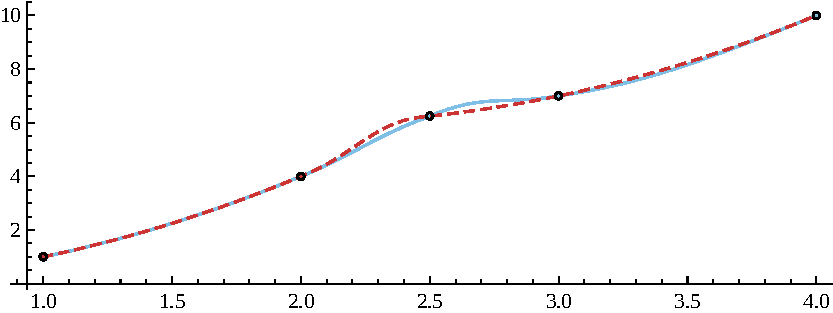
\includegraphics[width=.8\textwidth]{Figures/TOMS/1-sensitivity.pdf}
  \caption{A demonstration of the quadratic
  facet model's sensitivity to small data perturbations. This example is
  composed of two quadratic functions $f_1(x) = x^2$ over points $\{1$,
  $2$, $5/2\}$, and $f_2(x) = (x-2)^2 + 6$ over points $\{5/2$, $3$,
  $4\}$. Notably, $f_1(5/2) = f_2(5/2)$ and $f_1$, $f_2$ have the same
  curvature. Given the exact five data points seen above, the quadratic
  facet model produces the slope seen in the solid blue line at $x = 5/2$.
  However, by subtracting the value of $f_3$ $= \epsilon(x-2)^2$ from
  points at $x = 3$, $4$, where $\epsilon$ is the machine precision
  ($2^{-52}$ for an IEEE 64-bit real), the quadratic facet model produces
  the slope seen in the dashed red line at $x = 5/2$. This is the nature
  of a facet model and a side effect of associating data with local facets.}
  \label{splines:fig-1}
\end{figure}


\section{Performance and Applications}

This section contains graphs of sample {\tt MQSI} results given various
data configurations. Computation times for various problem sizes are also
provided. The files accompanying the subroutine {\tt MQSI} offer multiple
usages, namely {\tt sample\_main.f90} that demonstrates Fortran 2003 usage
and a command line interface {\tt cli.f90} that produces {\tt MQSI} estimates
for points in batches from data files.  Compilation instructions and the
full package contents are specified in the {\tt README} file.

\begin{figure}
  \centering
  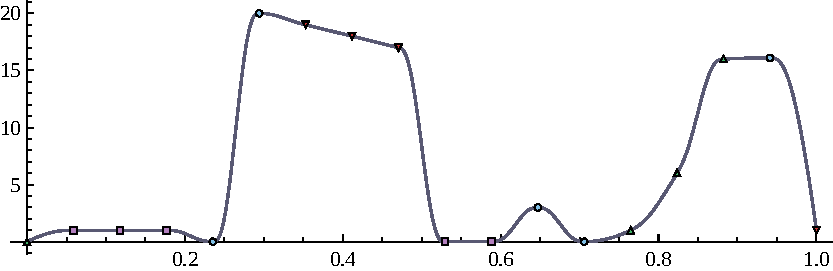
\includegraphics[width=.7\textwidth]{Figures/TOMS/2-piecewise-polynomial.pdf}
  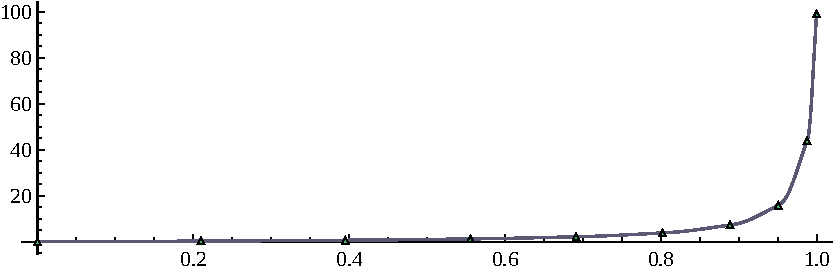
\includegraphics[width=.7\textwidth]{Figures/TOMS/3-large-tangent.pdf}
  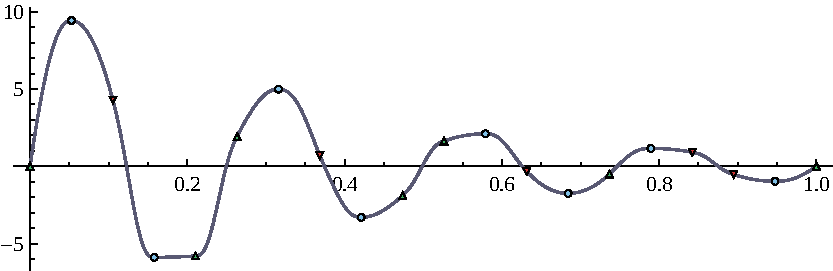
\includegraphics[width=.7\textwidth]{Figures/TOMS/4-signal-decay.pdf}
\caption{{\tt MQSI} results for three of the functions in the included test
suite. The {\it piecewise polynomial} function (top) shows the
interpolant capturing local linear segments, local flats, and
alternating extreme points. The {\it large tangent} (middle)
problem demonstrates outcomes on rapidly changing segments of data.
The {\it signal decay} (bottom) alternates between extreme values
of steadily decreasing magnitude.}
\label{splines:test_funcs}
\end{figure}

\begin{figure}
  \centering
  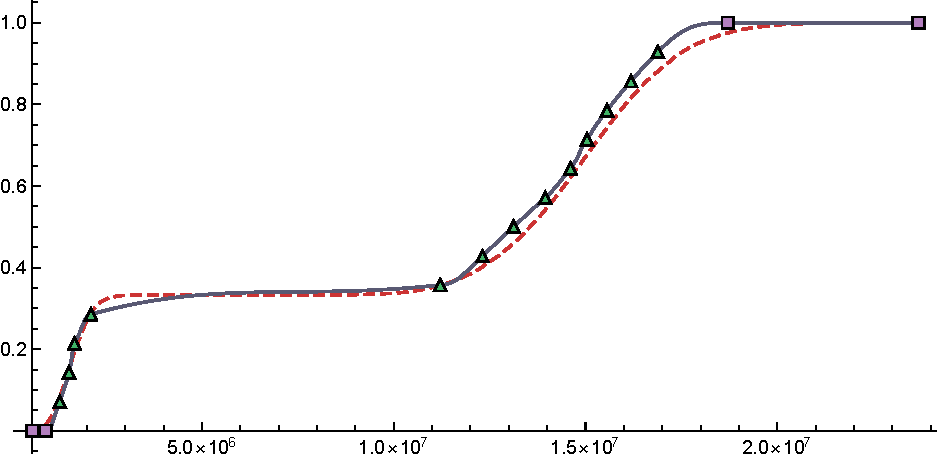
\includegraphics[width=.7\textwidth]{Figures/TOMS/5-real-data.pdf}
\caption{{\tt MQSI} results when approximating the cumulative distribution
function of system throughput (bytes per second) data for a computer
with a 3.2 GHz CPU performing file read operations from Cameron et al.
\cite{cameron2019moana}. The empirical distribution of 30 thousand throughput values is
shown in the red dashed line, while the solid line with stylized
markers denotes the approximation made with MQSI given equally spaced
empirical distribution points from a sample of size 100.}
\label{splines:cdf}
\end{figure}


\begin{figure}
  \centering
  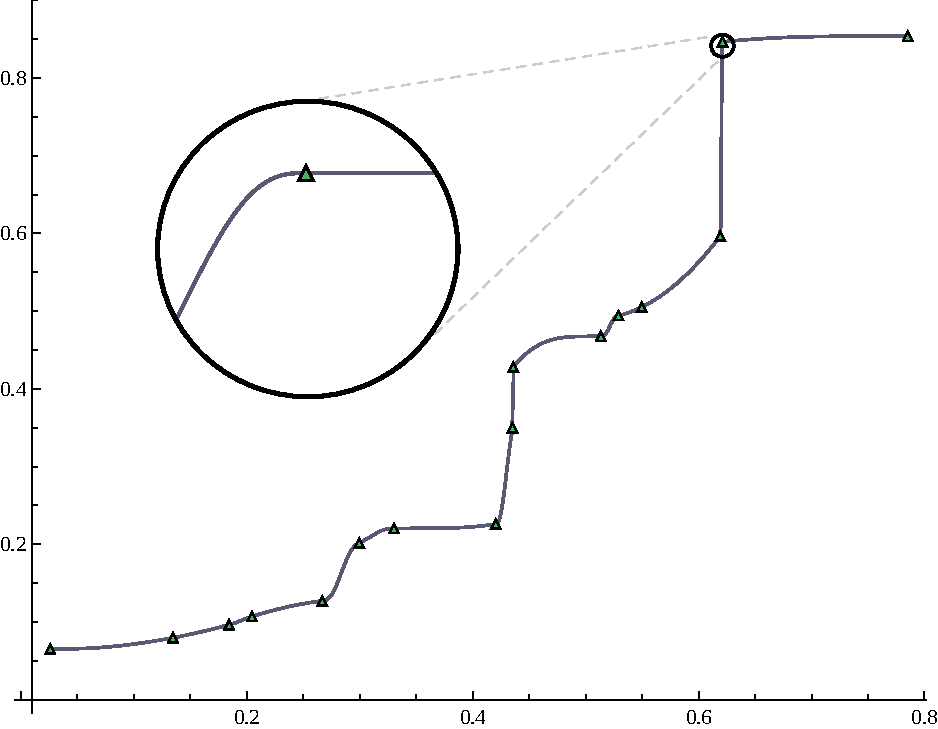
\includegraphics[width=.7\textwidth]{Figures/TOMS/6-random-monotone.pdf}
\caption{The {\it random monotone} test poses a particularly challenging
problem with large variations in slope. Notice that despite drastic
shifts in slope, the resulting monotone quintic spline interpolant
provides smooth and reasonable estimates to function values between data.}
\label{splines:random}
\end{figure}


Throughout, all visuals have points that are stylized by local
monotonicity conditions. Blue circles denote extreme points, purple
squares are in {\it flat} regions with no change in function value,
red down triangles are monotone decreasing, and green up triangles are
monotone increasing.

Figure \ref{splines:test_funcs} offers examples of the interpolating splines produced by the
routine {\tt MQSI} on various hand-crafted sets of data. These same
data sets are used for testing local installations in the provided
program {\tt test\_all.f90}. Notice that the quadratic facet model
perfectly captures the local linear segments of data in the piecewise
polynomial test for Figure \ref{splines:test_funcs}. Figure
\ref{splines:cdf} depicts an approximation of a
cumulative distribution function made by {\tt MQSI} on a computer
systems application by Cameron et al. \cite{cameron2019moana} that studies the
distribution of throughput (in bytes per second) when reading files
from a storage medium. Figure \ref{splines:random} provides a particularly difficult
monotone interpolation challenge using randomly generated monotone
data.

On a computer running MacOS 10.15.5 with a 2 GHz Intel Core i5 CPU, the
quadratic facet (Algorithm 1) takes roughly one microsecond ($10^{-6}$
seconds) per breakpoint, while the binary search (Algorithm 4) takes roughly
four microseconds per breakpoint; these times were generated from 100
repeated trials averaged over 14 different testing functions.  The vast
majority of execution time is spent solving the banded linear system of
equations in the routine {\tt FIT\_SPLINE} for the $B$-spline coefficients.
For large problems ($n > 100$) it would be faster to construct splines
over intervals independently (each interval requiring a $6 \times 6$ linear
system to be solved), however the single linear system is chosen here for
the decreased redundancy in the spline description.
